\documentclass{article}
\usepackage{hyperref}
\usepackage{graphicx}
\hypersetup{
    colorlinks=true,
    linkcolor=blue,
    filecolor=magenta,      
    urlcolor=cyan,
    pdftitle={Overleaf Example},
    pdfpagemode=FullScreen,
    }

\title{Running it all on Tomcat : \\ Geonetwork \& Geoserver}
\author{Advaith C A}

\begin{document}
    \maketitle
    \section*{Introduction}
        \hspace{1.5em}This article is written with the intention of it acting as a way to reproduce the results I achieved in getting Geonetwork and Geoserver running on my PC (A Windows device) using their web archive (\textit{WAR}) files on a tomcat server. I will provide a brief on the steps involved and the versions of the involved software, and the hardware I have used to get it all up and running. \par
        \hspace{1.5em}This will also contain information about setting up the WPS in geoserver so that the operations can be used. Some information on the creation of custom processes will also be provided.
    \section*{Hardware}
        \hspace{1.5em}The hardware specifications of my PC:
        \begin{itemize}
            \item AMD Ryzen 7 5800H with Radeon Graphics 3.20 GHz
            \item A dedicated RTX 3060 GPU
            \item 16 GB RAM
            \item 1 TB SSD (with roughly 260 GB Free space)
            \item Windows 11 v23H2
        \end{itemize}
    \section*{Versions of softwares used}
    \begin{itemize}
        \item Java 8
        \item Tomcat 9.0.89 (Supports running GeoNetwork 4.2.6)
        \item GeoNetwork 4.2.6 (Stable version)
        \item Geoserver 2.22.5 (Supports Java 8 SDK)
        \item Elasticsearch 7.17.15 (Supported by GeoNetwork 4.2.6)
    \end{itemize}
        \hspace{1.5em}The above versions were chosen after consulting the \href{https://docs.geonetwork-opensource.org\-/4.2/install-guide/}{documentation} of GeoNetwork.

    \section*{Steps}
        \subsection*{Downloading the files and their placements}
            \begin{enumerate}
                \item Download \href{https://www.oracle.com/java/technologies/javase/javase8u211-later-archive-downloads.html}{Java 8} and install it. Make sure that \textit{JAVA\_HOME} has been added to the Environment as a variable pointing to the installed JDK.
                \item Download the \href{https://dlcdn.apache.org/tomcat/tomcat-9/v9.0.89/bin/apache-tomcat-9.0.89.zip}{zip file} for Tomcat 9.0.89. Extract it to some location in your PC.
                \item Download the \href{https://sourceforge.net/projects/geonetwork/files/GeoNetwork_opensource/v4.2.6/geonetwork.war/download}{GeoNetwork.war} file for version 4.2.6. Add this file to the \emph{webapps} folder in the extracted Apache folder.
                \item Download the ElasticSearch \href{https://artifacts.elastic.co/downloads/elasticsearch/elasticsearch-7.17.15-windows-x86_64.zip}{zip file}. Extract it somewhere in your PC, preferrably somewhere near your previously extracted Apache folder to make navigation easier.
                \item Download GeoServer 2.22.5 \href{https://sourceforge.net/projects/geoserver/files/GeoServer/2.22.5/geoserver-2.22.5-war.zip}{WAR file}. It will be a zip file, extract and add the WAR file to webapps folder in the Apache directory.    
            \end{enumerate}
        \subsection*{Running the server}
            \begin{enumerate}
                \item Open a CMD or Terminal window in the \emph{bin} directory of Apache directory.
                \item Run the command \verb|startup.bat|
                \item Open another CMD or Terminal window in the \emph{bin} directory of the ElasticSearch directory.
                \item Run the command \verb|elasticsearch.bat|
            \end{enumerate}
        \subsection*{Troubleshooting}
            \begin{itemize}
                \item If after doing the above steps, nothing happens, please ensure that the versions are the same as that which I have used.
                \item If the search bar does not work in GeoNetwork, Edit the \emph{elasticsearch.yml} file the config directory of ElasticSearch, disable the security. (Usually the first uncommented line, make it false instead of true).
                \item If there are too many errors, just use WSL or spin up an Ubuntu virtual machine in Oracle VirtualBox.
            \end{itemize}
    \section*{WPS}
    \hspace{1.5em}I have opted to use GeoServer WPS as it integrates well with the GeoNetwork ecosystem, even though there is a huge learning curve to writing geoprocesses in Java.
        \subsection*{Setting up the geoserver WPS Plugin}
            \begin{enumerate}
                \item Download the \href{https://sourceforge.net/projects/geoserver/files/GeoServer/2.22.5/extensions/geoserver-2.22.5-wps-plugin.zip}{wps plugin} for geoserver 2.22.5.
                \item Extract the contents of this zip file to the \emph{WEB-INF\/lib} directory within the \emph{geoserver} directory that got created in the \emph{webapps} directory of the Apache server.
                \item Restart the Apache server using the command \verb|shutdown.bat| in the bin folder of the server directory.
                \item The WPS plugin will showup in the services section of the geoserver instance. 
            \end{enumerate}
        \subsection*{Getting the WPS in GeoNetwork}
        \hspace{1.5em}Copy the localhost address for the geoserver instance (http://localhost:8080/\-geoserver/ows, remove hyphens). Paste this into the search bar in the use WPS part in the Map. This will list out all the available processes.
        \begin{figure}[h!]
            \centering
            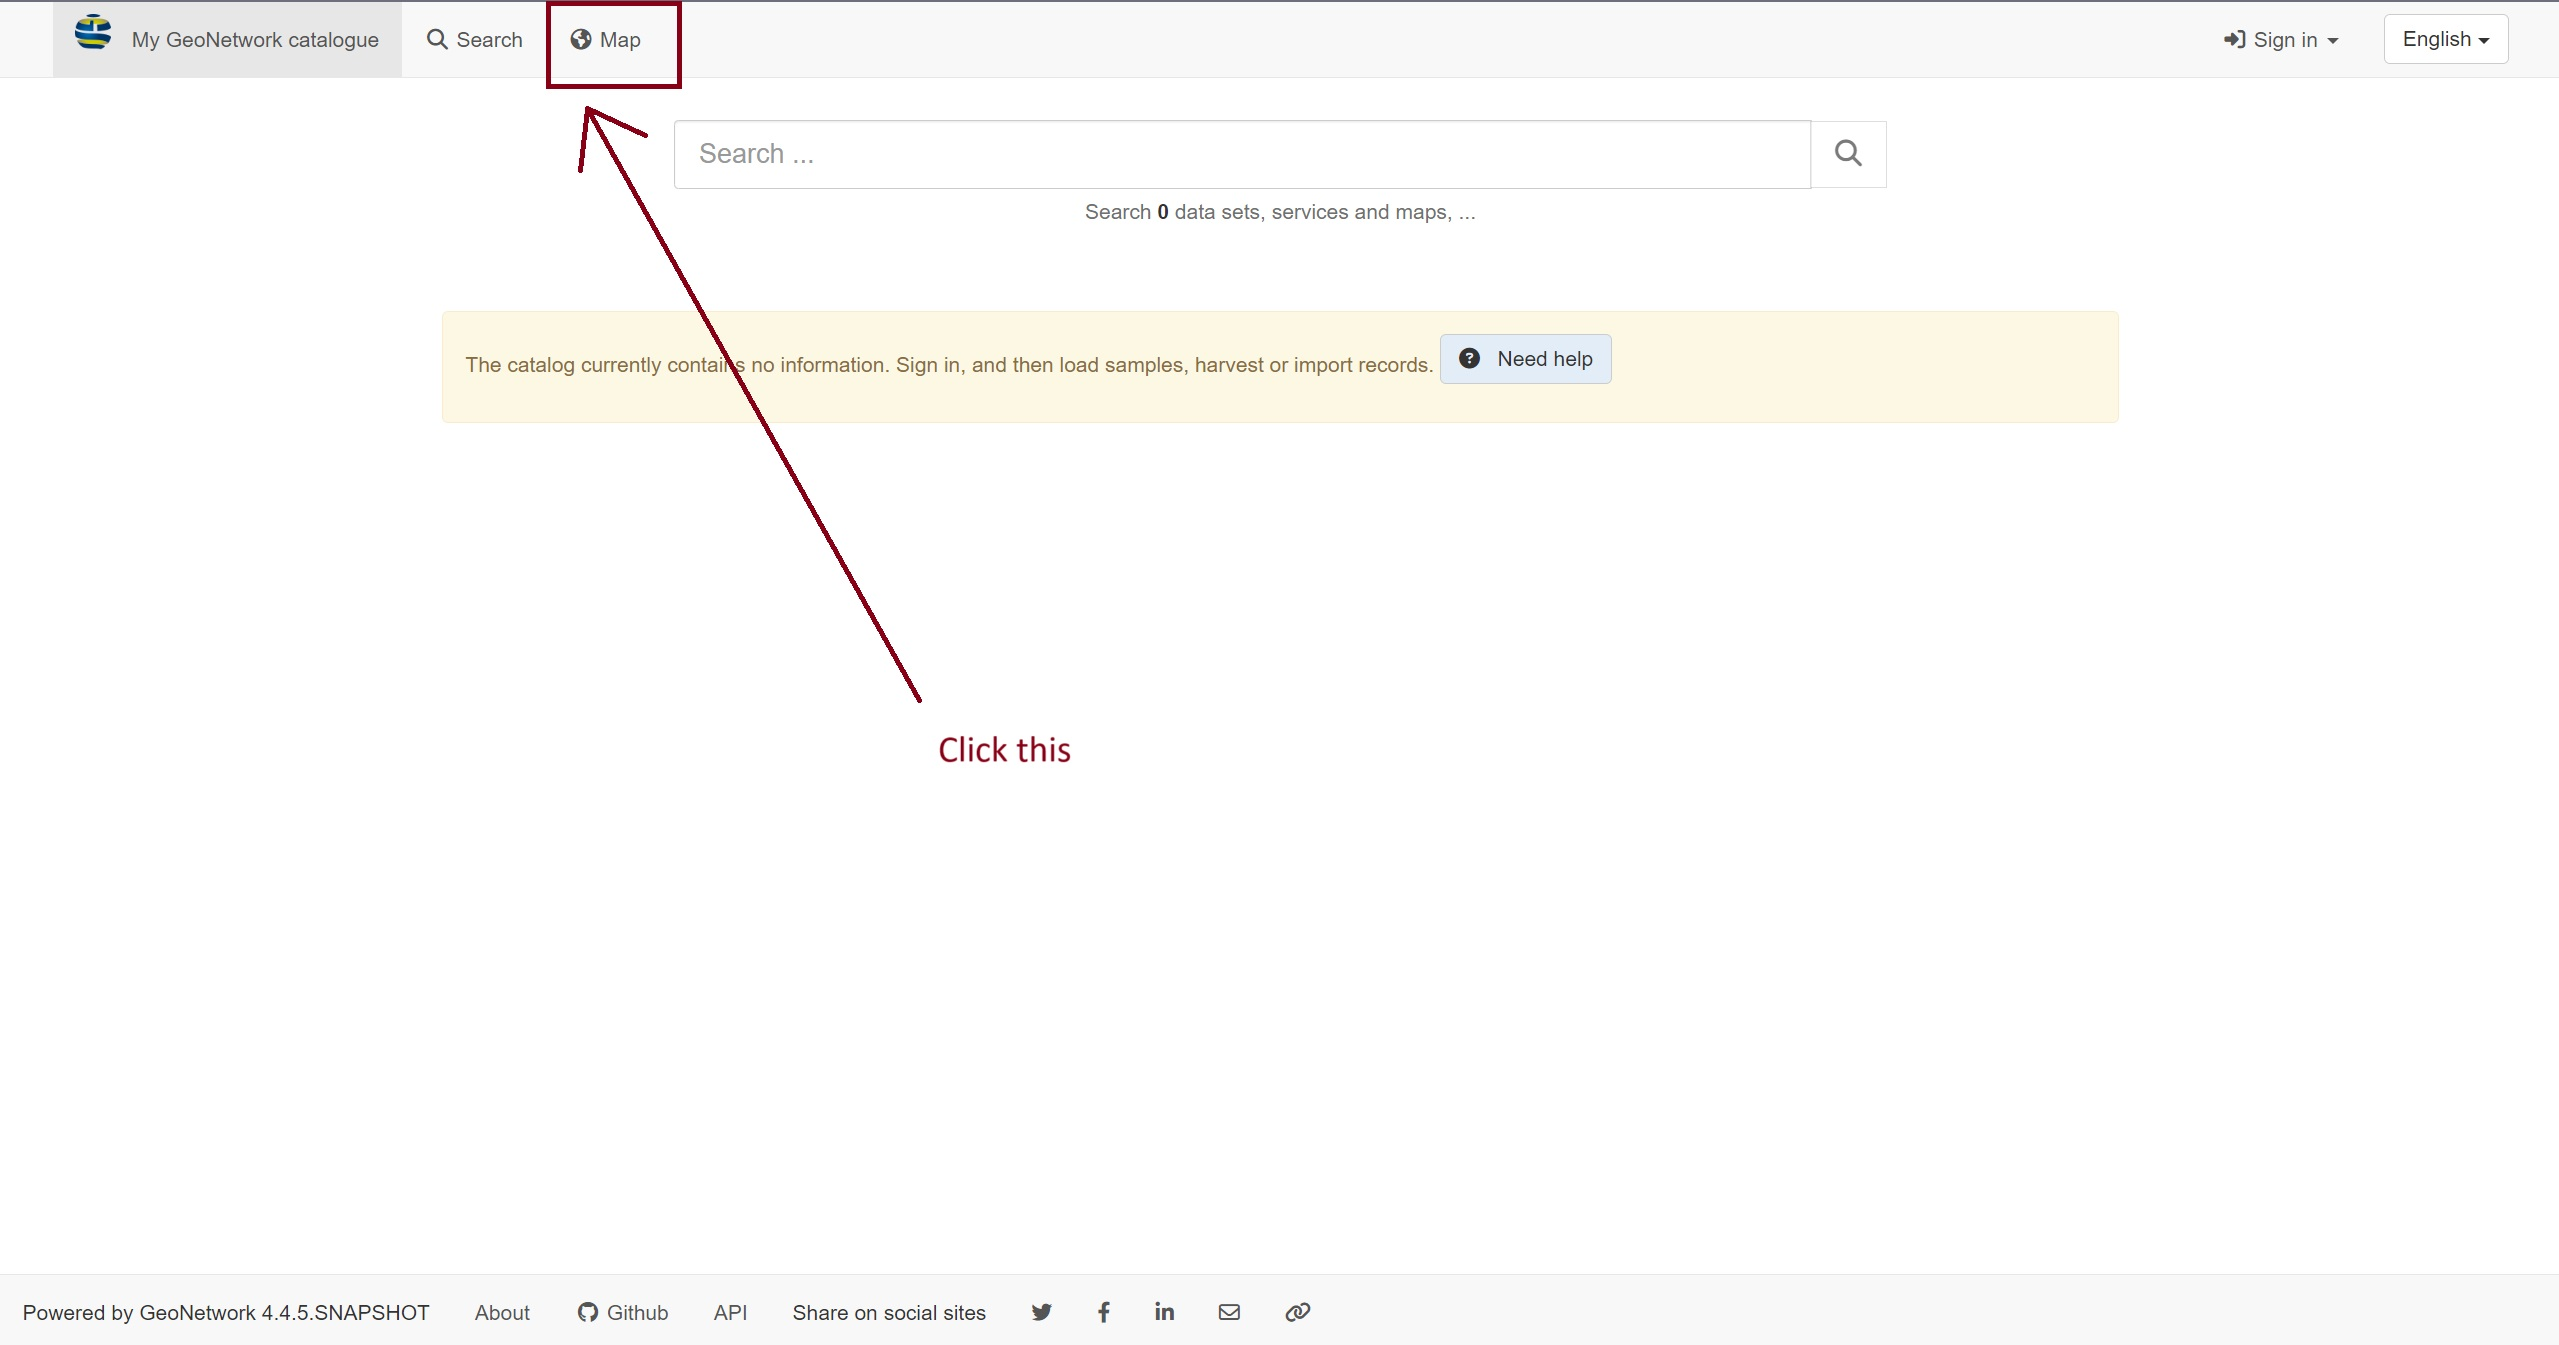
\includegraphics[width=\textwidth]{../images/Map.jpg}
            \caption{Click on the Map link to open the interactive Map.}
            \label{fig:fig-1}
        \end{figure}
        \begin{figure}[h!]
            \centering
            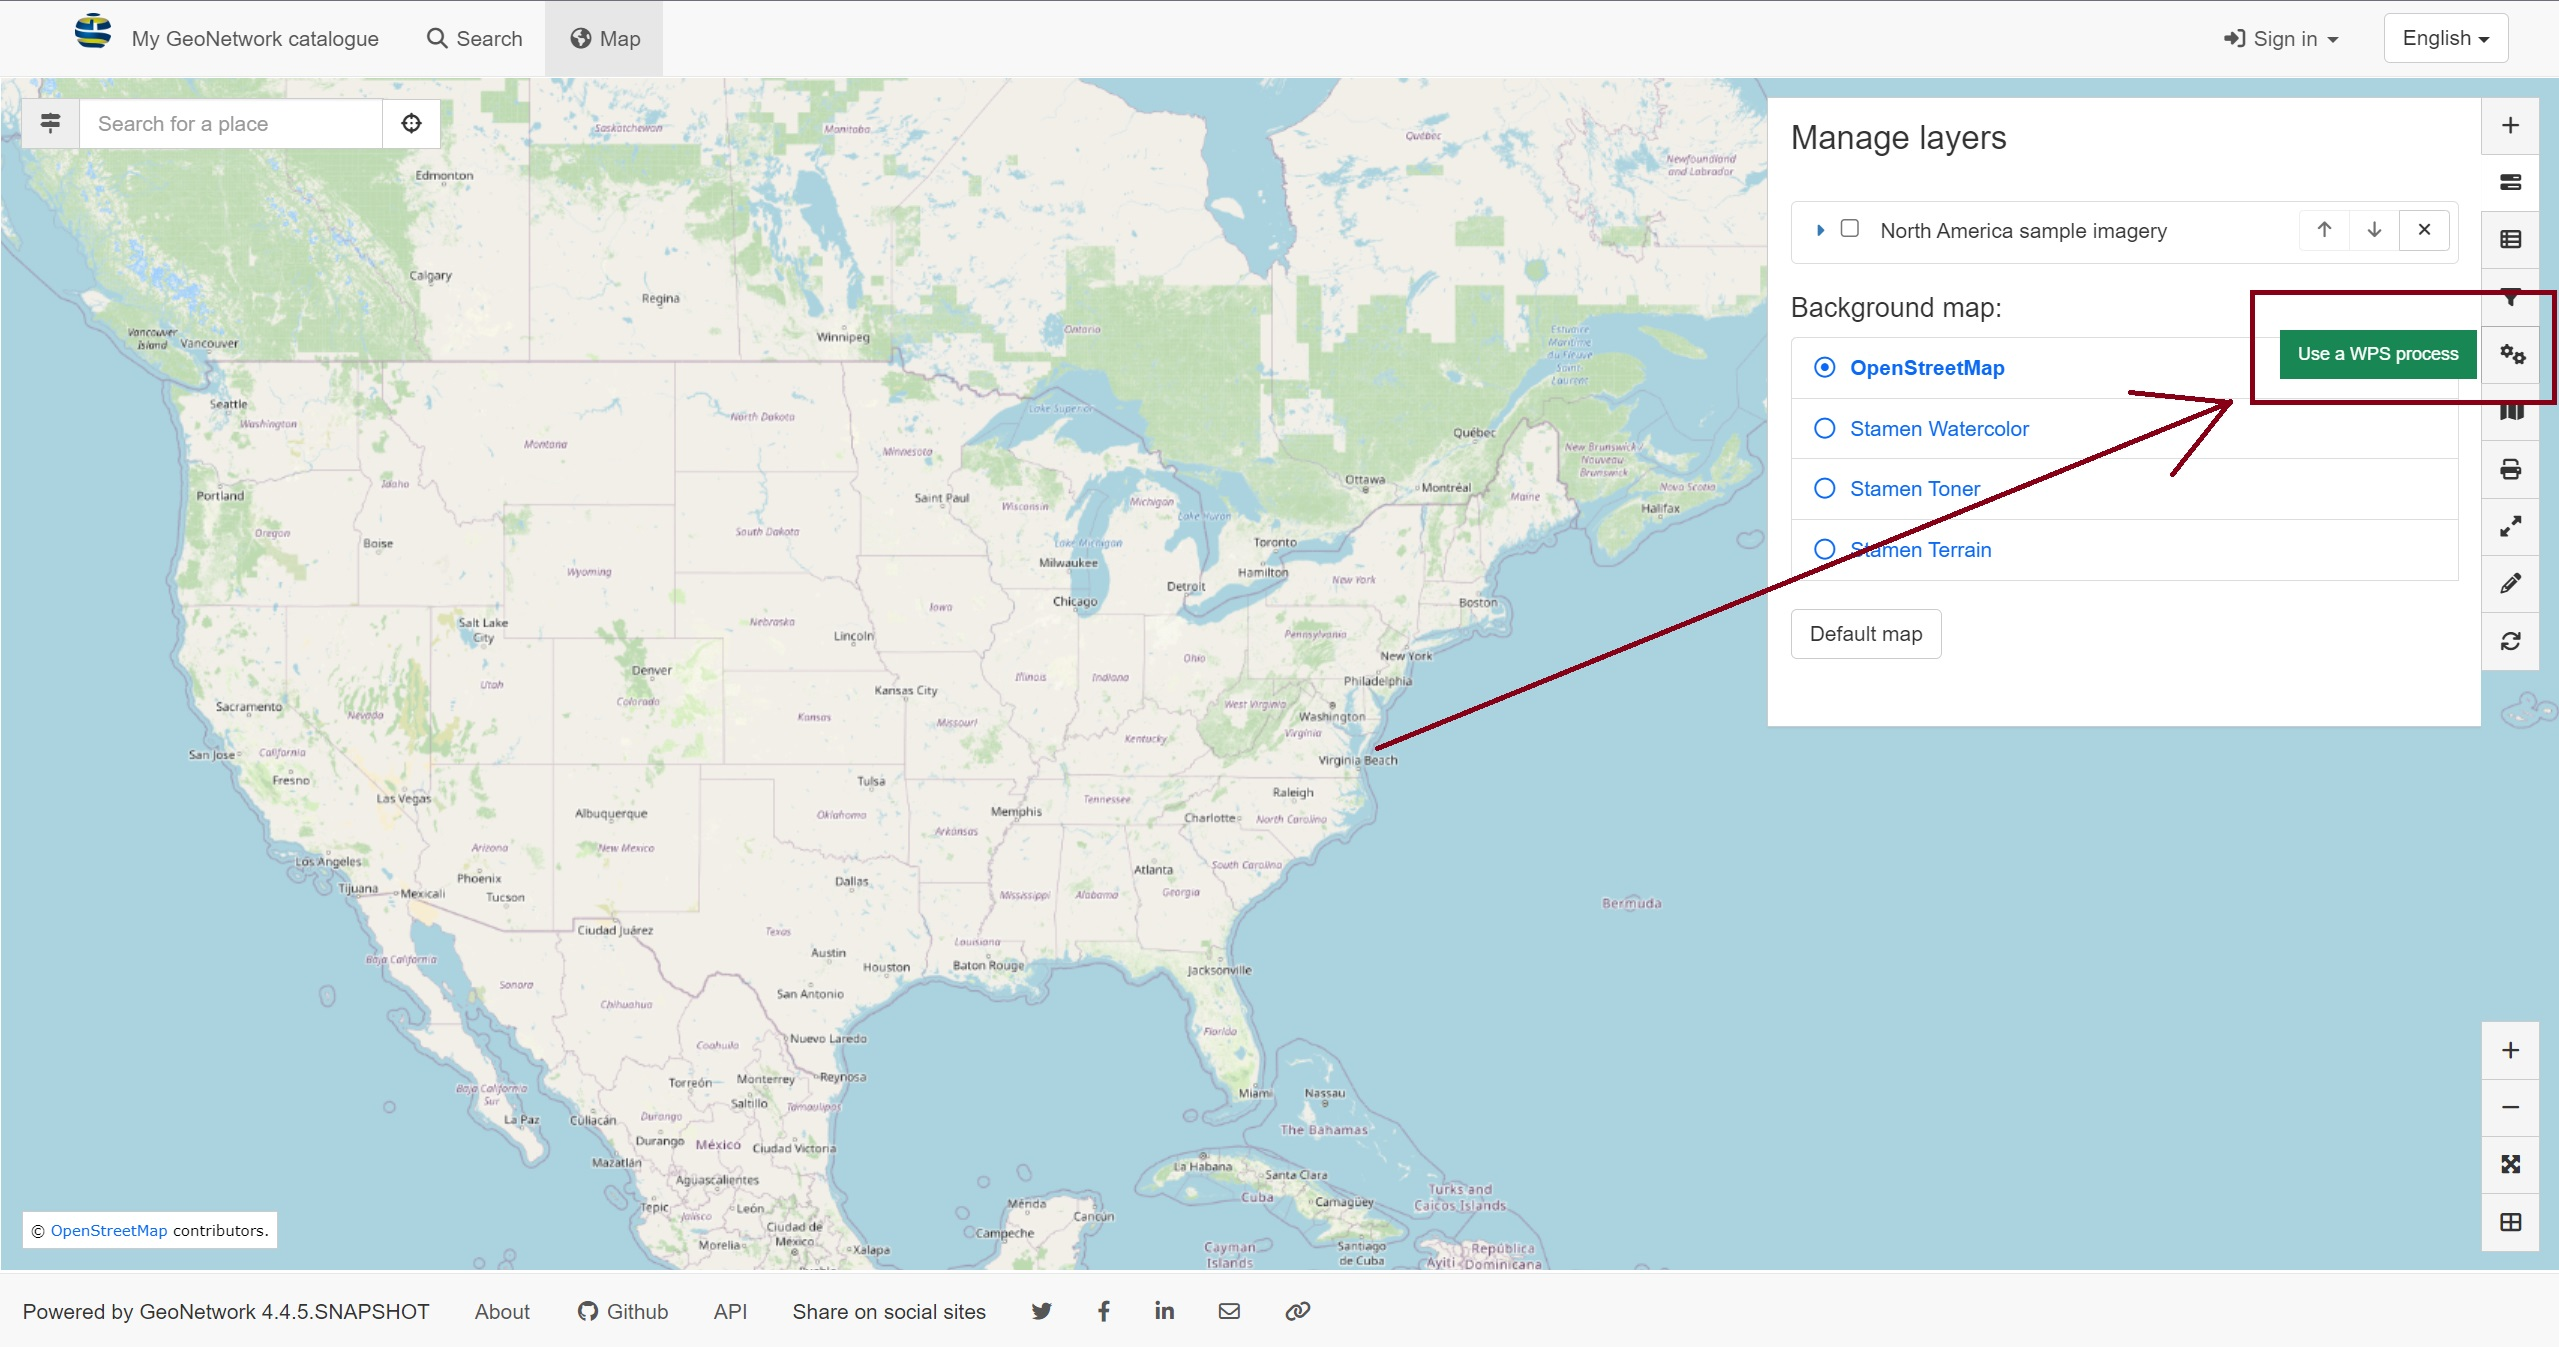
\includegraphics[width=\textwidth]{../images/Use WPS Process.jpg}
            \caption{Click on the Use WPS Process link}
            \label{fig:fig-2}
        \end{figure}
        \begin{figure}[h!]
            \centering
            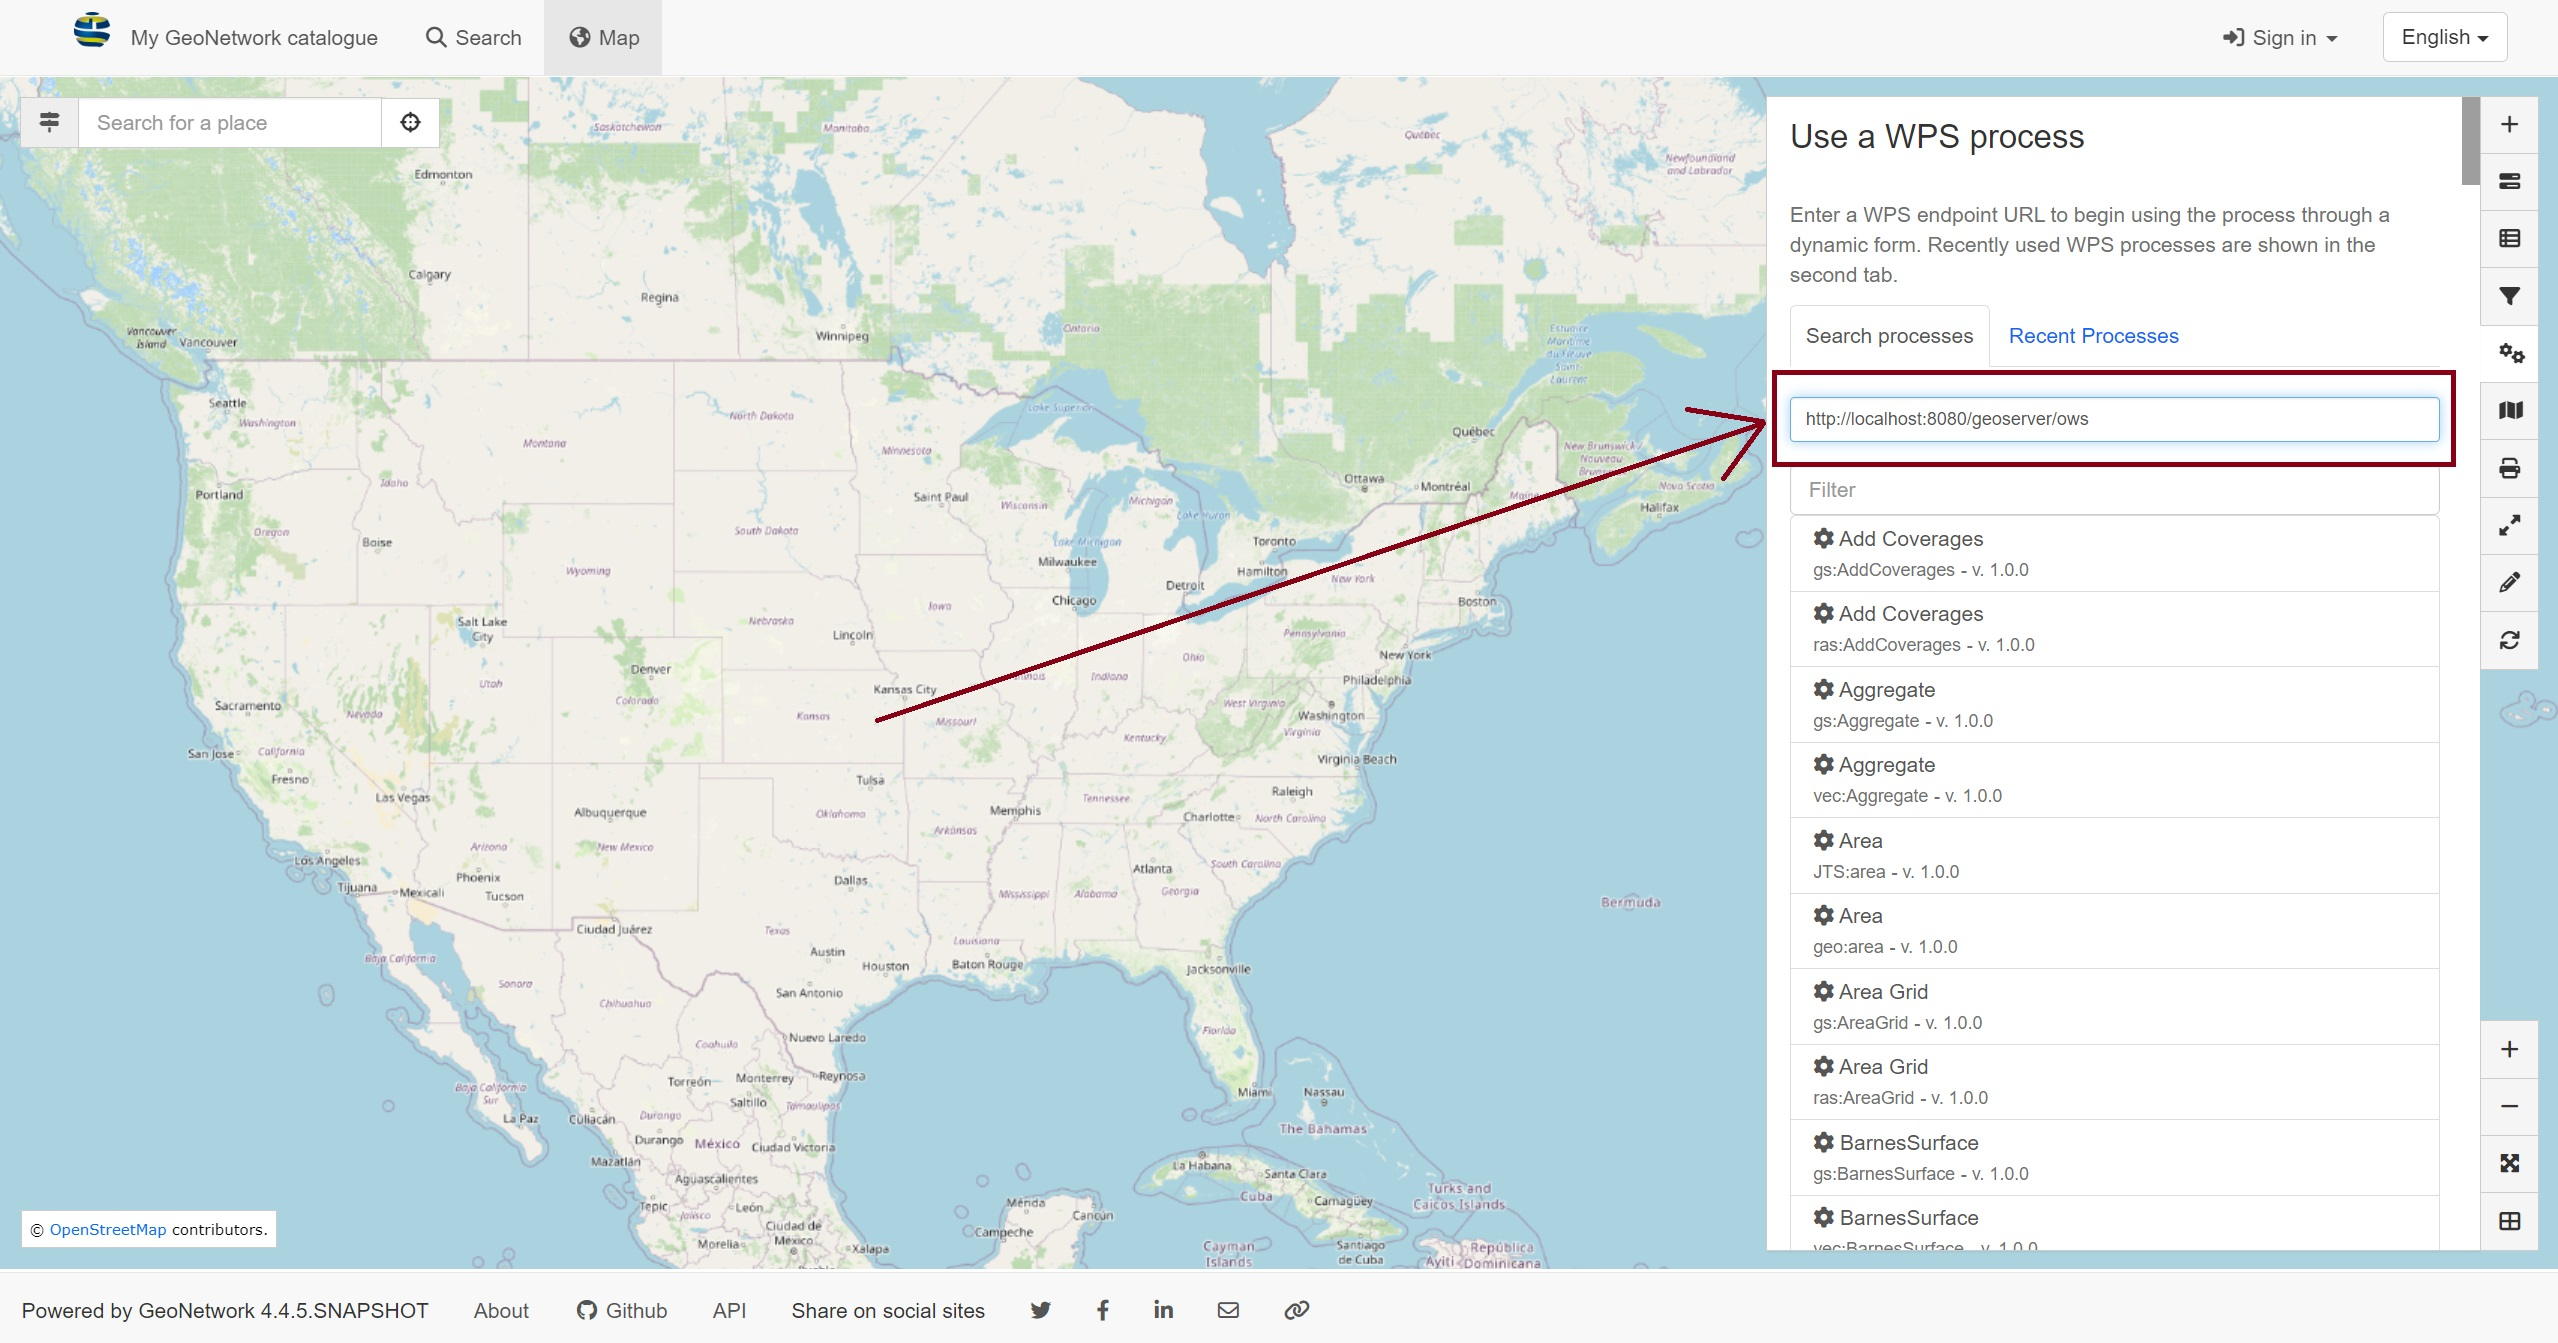
\includegraphics[width=\textwidth]{../images/Adding URL.jpg}
            \caption{Add URL and choose a process.}
            \label{fig:fig-3}
        \end{figure}
\end{document}